\documentclass[12pt, twoside]{article}
\usepackage[utf8]{inputenc}
\usepackage[english,russian]{babel}

\usepackage{amsthm}
\usepackage{a4wide}
\usepackage{graphicx}
\usepackage{caption}
\usepackage{amssymb}
\usepackage{amsmath}
\usepackage{mathrsfs}
\usepackage{euscript}
\usepackage{graphicx}
\usepackage{subfig}
\usepackage{caption}
\usepackage{color}
\usepackage{bm}
\usepackage{tabularx}
\usepackage{url}
\usepackage{adjustbox}

\usepackage{tikz}
\usetikzlibrary{bayesnet}
\usetikzlibrary{arrows}


\usepackage[toc,page]{appendix}

\usepackage{comment}
\usepackage{rotating}
\usepackage{multirow}

\DeclareMathOperator*{\argmax}{arg\,max}
\DeclareMathOperator*{\argmin}{arg\,min}

\newtheorem{theorem}{Теорема}
\newtheorem{lemma}[theorem]{Лемма}
\newtheorem{definition}{Определение}[section]

\newcommand*{\No}{No.}

\usepackage{autonum}

\begin{document}

\title{\bf Вероятностное обоснование дистилляции моделей машинного обучения \thanks{Работа выполнена при поддержке РФФИ и правительства РФ.}}
\date{}
\author{}
\maketitle

\begin{center}
\bf
А.\,В.~Грабовой\footnote{Московский физико-технический институт, grabovoy.av@phystech.edu}, В.\,В.~Стрижов\footnote{Московский физико-технический институт, strijov@phystech.edu}

\end{center}

{\centering\begin{quote}
\textbf{Аннотация:} 
Данная работа посвящена методам для понижения сложности модели при помощи дистилляции. Предлагается вероятностное обоснование методов для понижения сложности моделей машинного обучения путем дистилляции и привилегированного обучения. В работе показаны общие выводы для произвольной параметрической функции с заданой сигнатурой, а также показано теоретическое обоснование для частных случаев: линейной и логистической регрессии. Теоретические результаты анализируются в вычислительном эксперименте на синтетических выборках и реальных данных. В качестве реальных данных рассматривается выборка FashionMNIST и Twitter Sentiment Analysis.

\smallskip
\textbf{Ключевые слова}: дистилляция моделей, привилегированное обучения, выбор модели, байесовские методы.

\smallskip
\textbf{DOI}: 00.00000/00000000000000
\end{quote}
}

\section{Введение}
%Задача выбора модели машинного обучения является одной из самых распространенных и сложных задач текущего времени.
Повышение точности аппроксимации моделей в задачах машинного обучения влечет за собой усложнения моделей и как следствие снижает их интерпретируемость. Примером такого усложнения являются следующие модели: трансформеры~\cite{Vaswani2017}, BERT~\cite{Devlin2018}, ResNet~\cite{Kaiming2015} а также дальнейшее улучшение данной модели в виде ансамблирования. 

При построении модели машинного обучения используется два свойства: сложность модели и точность аппроксимации модели. Сложность влияет на время, которое модель требуется для принятия решения, а также на интерпретируемость модели, следовательно модель которая имеют меньшую сложность является более предпочтительной~\cite{bachteev2018}. С другой стороны точность аппроксимации модели нужно максимизировать. В данной работе рассматривается метод \textit{дистилляции} модели. Данные метод позволяет строить новые модели на основе ранее обученых моделей.

В работе~\cite{Hinton2015} рассматривается метод дистилляции моделей машиного обучения для задачи классификации. В работе проведен ряд экспериментов, в которых проводилась дистилляции моделей для разных задач машинного обучения. Эксперимент на выборке MNIST~\cite{mnist}, в котором избыточно сложностная нейросеть была дистиллирована в меньшую нейросеть. Эксперимент по Speech Recognition, в котором ансамбль моделей был \textit{дистиллирован} в одну модель. Также в работе~\cite{Hinton2015} был проведен эксперимент по обучению экспертных моделей на основе одной большой модели.

В работе~\cite{Vapnik2015} введено понятия \textit{привилегированной информации}~--- информации которая доступная только в момент обучения. В работе~\cite{Lopez2016} метод дистилляции~\cite{Hinton2015} используется вместе с привилегированным обучениям~\cite{Vapnik2015}. В предложенном методе на первом этапе обучается модель \textit{учителя} в пространстве привилегированной информации, после чего обучается модель \textit{ученика} в исходном признаковом пространстве используя \textit{дистилляцию}~\cite{Hinton2015}.

В данной работе предлагается рассмотреть общий подход дистилляции в рамках вероятностного подхода. Проводится обобщение на случай, когда привилегированная информация доступна не для всех объектов из обучающей выборки. Предлагается анализ и обобщение функции ошибки~\cite{Hinton2015, Lopez2016} в рамках вероятностного подхода. Также предлагается рассмотреть частные случаи для задач классификации и регрессии. 

В рамках вычислительного эксперимента анализируются модели, которые используют модель учителя при обучения  и модели, которые не используют модель учителя при обучения. Для анализа используются реальные выборки для задачи классификации изображений FashionMNIST~\cite{fashionmnist} и для задачи классификации текстов Twitter Sentiment Analysis~\cite{twiter2013}. В эксперименте использовалась выборка FashionMNIST, так-как выборка MNIST имеет хорошее качество аппроксимации даже для линейного классификатора. В рамках вычислительного эксперимента использовались модели разной сложности: линейные модели, полносвязная нейронная сеть, сверточная нейронная сеть~\cite{LeCun1989}, модель Bi-LSTM~\cite{Schmidhuber1997} и модель BERT~\cite{Devlin2018}.

\section{Постановка задачи обучения с учителем}
Пусть задано множество объектов~$\bm{\Omega}$ и множество целевых переменных~$\mathbb{Y}$:
\[
\label{eq:st:1}
\begin{aligned}
\bm{\Omega}, \quad \left|\bm{\Omega}\right| = m,
\end{aligned}
\]
где~$m$~--- число объектов, множество~$\mathbb{Y}=\{1,\cdots,K\}$ для задачи классификации, где~$K$ число классов, множество $\mathbb{Y}=\mathbb{R}$ для задачи регрессии.
Для множества~$\bm{\Omega}$ задано отображение в некоторое признаковое пространство~$\mathbb{R}^{n}$:
\[
\label{eq:st:phi}
\begin{aligned}
\varphi:\bm{\Omega} \to \mathbb{R}^{n},
\end{aligned}
\]
где~$n$ размерность признакового пространства. Обозначим~$\varphi(\bm{\Omega}) = \mathbf{X}$.
Пусть для объектов~$\bm{\Omega}^* \subset \bm{\Omega}$ задана привилегированная информация:
\[
\label{eq:st:phi*}
\begin{aligned}
\varphi^*:\bm{\Omega}^* \to \mathbb{R}^{n^*}, \quad \left|\bm{\Omega}^*\right| = m^*,
\end{aligned}
\]
где~$m^* \leq m$~--- число объектов с привилегированной информацией, $n^*$~--- число признаков в пространстве привилегированной информации. Обозначим~$\varphi^*(\bm{\Omega}^*) = \mathbf{X}^*$.

Множество индексов объектов, для которых известна привилегированная информация, обозначим~$\mathcal{I}$:
\[
\label{eq:st:3}
\begin{aligned}
\mathcal{I} = \{1 \leq i \leq m |~\text{для $i$-го объекта задана привилегированная информация}\},
\end{aligned}
\]
а множество индексов объектов, для которых не известна привилегированная информация, обозначим $\{1, \cdots, m\}\setminus \mathcal{I} = \bar{\mathcal{I}}$.

Пусть на множестве привилегированных признаков задана функция учителя~$\mathbf{f}\bigr(\mathbf{x}^*\bigr)$:
\[
\label{eq:st:4}
\begin{aligned}
\mathbf{f}:\mathbb{R}^{n^*} \to \mathbb{Y}^*,
\end{aligned}
\]
где~$\mathbb{Y}^*=\mathbb{Y}$ для задачи регрессии и $\mathbb{Y}^*$ является единичным симплексом~$\mathcal{S}_K$ в пространстве размерности~$K$ для задачи классификации. Обозначим ответы модели~$\mathbf{f}\bigr(\mathbf{x}^*_i\bigr)=\mathbf{s}_i$.  Получим ответы~$\mathbf{S}$ модели учителя~$\mathbf{f}$.

Требуется построить модель~$\mathbf{g}\bigr(\mathbf{x}\bigr)$ над множеством исходных признаков:
\[
\label{eq:st:5}
\begin{aligned}
\mathbf{g}:\mathbb{R}^{n} \to \mathbb{Y}^*.
\end{aligned}
\]
Пусть~$\mathbf{g}$ выбирается из некоторого множества функций:
\[
\label{eq:st:G}
\begin{aligned}
\mathcal{G} = \left\{\mathbf{g}| \mathbf{g}:\mathbb{R}^{n} \to \mathbb{Y}^*\right\},
\end{aligned}
\]
например для задачи классификации множество~$\mathcal{G}$ может быть параметрическим семейством функций линейных моделей $\mathcal{G} = \left\{\mathbf{g}\bigr(\mathbf{W}, \mathbf{x}\bigr)| \mathbf{g}\bigr(\mathbf{W}, \mathbf{x}\bigr) = \text{softmax}\bigr(\mathbf{W}\mathbf{x}\bigr)\right\}.$

\section{Постановка задачи: Хинтон \& Вапник}\label{state:hinton}
Рассмотрим описание метода предложеного в работах~\cite{Hinton2015, Lopez2016}. В рамках данных работ предполагается, что~$\mathcal{I} = \{1, 2, \cdots, m\}$. В работе~\cite{Hinton2015} решается задача классификации вида:
\[
    \mathcal{D} = \{\left(\mathbf{x}_i, y_i\right)\}_{i=1}^{m}, \qquad \mathbf{x}_i \in \mathbb{R}^{n}, \quad y_i \in \{1, \cdots, K\},
\]
где~$y_i$~--- это класс объекта, также будем обозначать~$\mathbf{y}_i$ one hot вектором для класса~$y_i$.

В данной постановке рассматривается параметрическое семейство функций:
\[
\label{eq:G:set:cl}
\mathcal{G}_{\text{cl}} = \left\{\mathbf{g}| \mathbf{g} = \text{softmax}\bigr(\mathbf{z}\bigr(\mathbf{x}\bigr)/T\bigr), \quad \mathbf{z}: \mathbb{R}^n \to \mathbb{R}^K \right\},
\]
где~$\mathbf{z}$~--- это дифференцируемая параметрическая функция, $T$~--- параметр температуры. В качестве модели учителя~$\mathbf{f}$ рассматривается функция из множества~$\mathcal{F}_{\text{cl}}$:
\[
\label{eq:F:set:cl}
\mathcal{F}_{\text{cl}} = \left\{\mathbf{f}| \mathbf{f} = \text{softmax}\bigr(\mathbf{v}\bigr(\mathbf{x}\bigr)/T\bigr), \quad \mathbf{v}: \mathbb{R}^n \to \mathbb{R}^K \right\},
\]
где~$\mathbf{v}$~--- это дифференцируемая параметрическая функция, $T$~--- параметр температуры. 

Параметр температуры~$T$ имеет следующие свойства:
\begin{enumerate}
    \item[1)] при~$T\to 0$ получаем one hot вектора;
    \item[1)] при~$T\to \infty$ получаем равновероятные классы.
\end{enumerate}

Функция потерь в которой учитывается перенос информации от модели учителя~$\mathbf{f}$ к модели ученика~$\mathbf{g}$ имеет следующий вид:
\[
\label{eq:hinton:1}
\begin{aligned}
   \mathcal{L}\bigr(\mathbf{g}\bigr) = &-\sum_{i=1}^{m}\underbrace{{\sum_{k=1}^{K}y^k_i\log\mathbf{g}\bigr(\mathbf{x}_i\bigr)\bigr|_{T=1}}}_{\text{исходная функция потерь}}\\
   &-\sum_{i=1}^{m}\underbrace{{\sum_{k=1}^{K}\mathbf{f}\bigr(\mathbf{x}_i\bigr)\bigr|_{T=T_0}\log\mathbf{g}\bigr(\mathbf{x}_i\bigr)\bigr|_{T=T_0}}}_{\text{слагаемое дистилляция}},
\end{aligned}
\]
где $\cdot\bigr|_{T=t}$~--- обозначает, что параметр температуры~$T$ в предыдущей функции равно~$t$.

Получаем оптимизационную задачу:
\[
\label{eq:hinton:opt}
\begin{aligned}
   \hat{\mathbf{g}} = \arg\min_{\mathbf{g} \in \mathcal{G}_{\text{cl}}} &-\sum_{i=1}^{m}{\sum_{k=1}^{K}y^k_i\log\mathbf{g}\bigr(\mathbf{x}_i\bigr)\bigr|_{T=1}}\\
   &-\sum_{i=1}^{m}{\sum_{k=1}^{K}\mathbf{f}\bigr(\mathbf{x}_i\bigr)\bigr|_{T=T_0}\log\mathbf{g}\bigr(\mathbf{x}_i\bigr)\bigr|_{T=T_0}}.
\end{aligned}
\]

В работе~\cite{Lopez2016} метод~\cite{Hinton2015} имеет обобщение. Решение задачи оптимизации~\eqref{eq:hinton:opt} зависит от модели учителя~$\mathbf{f}$, только через вектор ответов учителя. Следовательно признаковые пространства учителя и ученика могут различатся. В этом случае получаем следующую постановку задачи:
\[
    \mathcal{D} = \left\{\left(\mathbf{x}_i, \mathbf{x}^*_i, y_i\right)\right\}_{i=1}^{m}, \qquad \mathbf{x}_i \in \mathbb{R}^{n}, \quad \mathbf{x}^*_i \in \mathbb{R}^{n^*}, \quad y_i \in \{1, \cdots, K\},
\]
где~$\mathbf{x}_i$ это информация доступна на этапах обучения и контроля, а $\mathbf{x}^*_i$ это информация доступна только на этапе обучения.

В данном случае в качестве функции учителя выбирается функция~$\mathbf{f}$ не из множества~$\mathcal{F}_{cl}$, а из множества~$\mathcal{F}_{cl}^*$:
\[
\label{eq:F:set:cl:priv}
\mathcal{F}_{\text{cl}}^* = \left\{\mathbf{f}| \mathbf{f} = \text{softmax}\bigr(\mathbf{v}^*\bigr(\mathbf{x}^*\bigr)/T\bigr), \quad \mathbf{v}^*: \mathbb{R}^{n^*} \to \mathbb{R}^K \right\},
\]
где~$\mathbf{v}^*$~--- это дифференцируемая параметрическая функция, $T$~--- параметр температуры. 

Требуется построить модель, которая использует привилегированную информацию $\mathbf{x}^*_i$ при обучении. Для этого рассмотрим двухэтапную модель обучения предложенную в работе~\cite{Lopez2016}:
\begin{enumerate}
    \item[1)] выбираем оптимальную модель учителя $\mathbf{f} \in \mathcal{F}_{\text{cl}}^*$;
    \item[2)] выбираем оптимальную модель ученика $\mathbf{g} \in \mathcal{G}_{\text{cl}}$ используя дистилляцию~\cite{Hinton2015}. 
\end{enumerate}

Модель ученика~--- это функция, которая минимизирует \eqref{eq:hinton:1}. Модель учителя~--- это функция, которая минимизирует Cross Entropy Loss:
\[
\label{eq:hinton.2}
\begin{aligned}
   \mathcal{L}\bigr(\mathbf{f}\bigr) = &-\sum_{i=1}^{m}{{\sum_{k=1}^{K}y^k_i\log\mathbf{f}\bigr(\mathbf{x}^*_i\bigr)}}.
   \end{aligned}
\]

\section{Постановка задачи: вероятностный подход}
\subsection{Метод максимального правдоподобия}
Для поиска~$\hat{\mathbf{g}}$ воспользуемся методом максимального правдоподобия:
\[
\label{eq:st:6}
\begin{aligned}
p\bigr(\mathbf{Y}|\mathbf{X}, \mathbf{g}\bigr) = \prod_{i=1}^{N}p\bigr(\mathbf{y}_{i}|\mathbf{x}_i, \mathbf{g}\bigr).
\end{aligned}
\]
В качестве~$\hat{\mathbf{g}}$ выбирается функция, которая максимизирует правдоподобие модели~\eqref{eq:st:6}:
\[
\label{eq:st:7}
\begin{aligned}
\hat{\mathbf{g}} = \arg\max_{\mathbf{g}\in \mathcal{G}} \prod_{i=1}^{N}p\bigr(\mathbf{y}_{i}|\mathbf{x}_i, \mathbf{g}\bigr),
\end{aligned}
\]
где множество~$\mathcal{G}$ задается~\eqref{eq:st:G}.
\subsection{Подход дистилляции модели учителя в модель ученика}
Рассмотрим вероятностную постановку, в которой должны быть выполнены ограничения:
\begin{enumerate}
	\item[1)] для всех $\omega \in \bm{\Omega}^*$ элементы $\mathbf{y}(\omega)$ и $\mathbf{s}(\omega)$ являются зависимыми величинами, так как ответы учителя должны коррелировать с истинными ответами;
	\item[2)] если $|\bm{\Omega}^*|=0$ то решение должно соответствовать решению~\eqref{eq:st:7};
	\item[3)] рассмотрим параметр~$\lambda\in[0,1]$ как уровень доверия к ответам модели~$\mathbf{f}$, которая задана в~\eqref{eq:st:4}.
\end{enumerate}

Рассмотрим совместное правдоподобие истинных меток и меток учителя:
\[
\label{eq:st:8}
\begin{aligned}
p\bigr(\mathbf{Y}, \mathbf{S}|\mathbf{X}, \mathbf{g}, \mathcal{I}, \lambda\bigr)=\prod_{i\not\in \mathcal{I}}p\bigr(\mathbf{y}_i|\mathbf{x}_i, \mathbf{g}\bigr)\prod_{i\in \mathcal{I}}p\bigr(\mathbf{y}_i, \mathbf{s}_i|\mathbf{x}_i, \mathbf{g}, \lambda\bigr).
\end{aligned}
\]
Рассмотрим~$p\bigr(\mathbf{y}_i, \mathbf{s}_i|\mathbf{X}, \mathbf{g}, \lambda\bigr)$ следующего вида:
\[
\label{eq:st:bernuli}
\begin{aligned}
p\bigr(\mathbf{y}_i, \mathbf{s}_i|\mathbf{X}, \mathbf{g}, \lambda\bigr) = p\bigr(\mathbf{y}_i|\mathbf{x}_i, \mathbf{g}\bigr)\prod_{i\in \mathcal{I}}\bigr(\mathbf{s}_i|\mathbf{y}_i, \mathbf{x}_i, \mathbf{g}\bigr)
\end{aligned}
\]
Подставляя выражения~\eqref{eq:st:bernuli} в~\eqref{eq:st:8} получаем.
\[
\label{eq:st:9}
\begin{aligned}
p\bigr(\mathbf{Y}, \mathbf{S}|\mathbf{X}, \mathbf{g}, \mathcal{I}, \lambda\bigr)=\prod_{i\not\in \mathcal{I}}p\bigr(\mathbf{y}_i|\mathbf{x}_i, \mathbf{g}\bigr)\prod_{i\in \mathcal{I}}p\bigr(\mathbf{y}_i|\mathbf{x}_i, \mathbf{g}\bigr)\prod_{i\in \mathcal{I}}p\bigr(\mathbf{s}_i|\mathbf{y}_i, \mathbf{x}_i, \mathbf{g}\bigr).
\end{aligned}
\]
Заметим, что~$\mathbf{y}_i$ и~$\mathbf{s}_i$ зависимы только через переменную~$\mathbf{x}_i$, тогда~$p\bigr(\mathbf{s}_i|\mathbf{y}_i, \mathbf{x}_i, \mathbf{g}\bigr)=p\bigr(\mathbf{s}_i|\mathbf{x}_i, \mathbf{g}\bigr)$. Получаем совместное правдоподобие:
\[
\label{eq:st:10}
\begin{aligned}
p\bigr(\mathbf{Y}, \mathbf{S}|\mathbf{X}, \mathbf{g}, \mathcal{I}, \lambda\bigr)=\prod_{i\not\in \mathcal{I}}p\bigr(\mathbf{y}_i|\mathbf{x}_i, \mathbf{g}\bigr)\prod_{i\in \mathcal{I}}p\bigr(\mathbf{y}_i|\mathbf{x}_i, \mathbf{g}\bigr)\prod_{i\in \mathcal{I}}p\bigr(\mathbf{s}_i|\mathbf{x}_i, \mathbf{g}\bigr).
\end{aligned}
\]
Используя~\eqref{eq:st:10} получаем следующую оптимизационную задачу для поиска~$\hat{\mathbf{g}}$
\[
\label{eq:st:11}
\begin{aligned}
\hat{\mathbf{g}} = \arg\max_{\mathbf{g}\in \mathcal{G}} \prod_{i\not\in \mathcal{I}}p\bigr(\mathbf{y}_i|\mathbf{x}_i, \mathbf{g}\bigr)\prod_{i\in \mathcal{I}}p\bigr(\mathbf{y}_i|\mathbf{x}_i, \mathbf{g}\bigr)\prod_{i\in \mathcal{I}}p\bigr(\mathbf{s}_i|\mathbf{x}_i, \mathbf{g}\bigr).
\end{aligned}
\]
Для удобства, будем минимизировать логарифм, тогда из~\eqref{eq:st:11} получаем:
\[
\label{eq:st:12}
\begin{aligned}
\hat{\mathbf{g}} = \arg\max_{\mathbf{g}\in \mathcal{G}} \sum_{i\not\in \mathcal{I}}\log p\bigr(\mathbf{y}_i|\mathbf{x}_i, \mathbf{g}\bigr) + \left(1-\lambda\right)\sum_{i\in \mathcal{I}}\log p\bigr(\mathbf{y}_i|\mathbf{x}_i, \mathbf{g}\bigr) + \lambda\sum_{i\in \mathcal{I}}\log p\bigr(\mathbf{s}_i|\mathbf{x}_i, \mathbf{g}\bigr),
\end{aligned}
\]
где параметр~$\lambda$ введен для взвешивания ошибок на истинных ответах и ошибок относительно ответов учителя.

\begin{figure}
\begin{center}
  \tikz{
    % nodes
     \node[obs] (y) {$y_i$};%
     \factor[left=of y] {y-f} {below:$\text{Cat}$} {} {} ; %
     \node[det, left=of y] (g) {$\mathbf{g}$}; %
     
     \node[obs, below=of g] (s) {$\mathbf{s}_i$};%
     
     \node[obs, left=of g] (x) {$\mathbf{x}_i$};%
    % plates
     \plate {xy} {(x) (y) (g)} {$m$}; %
     \plate {xs} {(x) (s) (g)} {$m^*$}; %
    % edges
    \edge[-] {x} {g} ;
    \edge {g} {y} ; %
    \edge {g} {s} ; %
 }
\end{center}
\caption{Общий вид модели в формате plate notation.}
\label{fg:st:plate}
\end{figure}

На рис.~\ref{fg:st:plate} показан общий вид вероятностной модели в графовой нотации. Для каждой реализации функции $\mathbf{g}$ данный вид изменяется. На рис~\ref{fg:ex:synt:plate} показана более подробная реализация в случае, когда модель~$\mathbf{g}$ это линейная модель.

\section{Частные случаи обучения с учителем}
\subsection{Случай классификации}
Для задачи многоклассовой классификации рассматриваются следующие вероятностные предположения:
\begin{enumerate}
\label{st:class:1}
	\item[1)] рассматривается функция учителя $\mathbf{f}\in\mathcal{F}_{\text{cl}}^{*}$;
	\item[2)] рассматривается функция ученика следующего вида $\mathbf{g}\in\mathcal{G}_{\text{cl}}$;
	\item[3)] для истинных меток рассмотривается категориальное распределение, задаваемое своей плотностью $p\bigr(y|\mathbf{x}, \mathbf{g}\bigr) = \text{Cat}\bigr(\mathbf{g}\bigr(\mathbf{x}\bigr)\bigr)$, где $\mathbf{g}\bigr(\mathbf{x}\bigr)\bigr)$ задает вероятность каждого класса;
	\item[4)] для меток учителя рассматривается плотность распределения
\[
\label{reg:dist}
\begin{aligned}
	p\bigr(\mathbf{s}|\mathbf{x}, \mathbf{g}\bigr) = C\prod_{k=1}^{K}g_k\bigr(\mathbf{x}\bigr)^{s^k}.
\end{aligned}
\]
\end{enumerate}
\begin{theorem}
\label{theorem:st:dist}
Пусть для всех $k$ выполняется $1 > 1- \varepsilon > g_k\bigr(\mathbf{x}\bigr) > \varepsilon > 0,$ тогда при 
\[
C=\left(-1\right)^{K}\frac{K^{K/2}}{2^{K(K-1)/2}}\prod_{k=1}^{K}g_k\bigr(\mathbf{x}\bigr)\log g_k\bigr(\mathbf{x}\bigr)
\]
функция $p\bigr(\mathbf{s}|\mathbf{x}, \mathbf{g}\bigr)$ определенная в~\eqref{reg:dist} является плотностью распределения.
\end{theorem}
\begin{proof}
	\item[1)] Покажем, что для произвольного $\mathbf{s} \in \mathcal{S}_K$ выполняется $p\bigr(\mathbf{s}|\mathbf{x}, \mathbf{g}\bigr) \geq 0$. Заметим, что для всех~$k$ выполняется, что~$\log g_k\bigr(\mathbf{x}\bigr) < 0,$ тогда
\[
\begin{aligned}
	C=\underbrace{\frac{K^{K/2}}{2^{K(K-1)/2}}}_{>0}\prod_{k=1}^{K}\underbrace{g_k\bigr(\mathbf{x}\bigr)}_{>\varepsilon}\underbrace{\left(-\log g_k\bigr(\mathbf{x}\bigr)\right)}_{>0} > 0,
\end{aligned}
\]
тогда с учетом того, что~$g_k\bigr(\mathbf{x}\bigr) >0$ и~$C>0$ получаем, что $p\bigr(\mathbf{s}|\mathbf{x}, \mathbf{g}\bigr) \geq 0$.
	\item[2)] Покажем, что интеграл по всему пространству объектов~$\mathcal{S}_K$ является конечным:
	\[
	\label{theorem:st:dist:eq:1}
	\begin{aligned}
		\int_{\mathcal{S}_K}p\bigr(\mathbf{s}|\mathbf{x}, \mathbf{g}\bigr)ds &= \int_{\mathcal{S}_K}\prod_{k=1}^{K}g_k\bigr(\mathbf{x}\bigr)^{s^k}ds = \prod_{k=1}^{K}\int_{\mathcal{S}_K}g_k\bigr(\mathbf{x}\bigr)^{s^k}ds\\ 
		& = \prod_{k=1}^{K}\int_{0}^{1}\frac{r^{K-1}\sqrt{K}}{\left(K-1\right)!\sqrt{2^{K-1}}}g_k\bigr(\mathbf{x}\bigr)^{r}dr = \prod_{k=1}^{K}\underbrace{\frac{\sqrt{K}}{\left(K-1\right)!\sqrt{2^{K-1}}}}_{D}\int_{0}^{1}r^{K-1}g_k\bigr(\mathbf{x}\bigr)^{r}dr \\
		& = D^K\prod_{k=1}^{K} \int_{0}^{1}r^{K-1}\exp\bigr(r\log g_k\bigr(\mathbf{x}\bigr)\bigr)dr \\
		& = \left(-D\right)^K\prod_{k=1}^{K}\log g_k\bigr(\mathbf{x}\bigr)\left(\Gamma\bigr(K\bigr) - \Gamma\bigr(K, -\log g_k\bigr(\mathbf{x}\bigr)\bigr)\right) \\
		& = \left(-D\right)^K\left(K-1\right)!^K\prod_{k=1}^{K}\log g_k\bigr(\mathbf{x}\bigr)\left(1 -g_k\bigr(\mathbf{x}\bigr) \exp_{K-1}\bigr(-\log g_k\bigr(\mathbf{x}\bigr)\bigr)+g_k\bigr(\mathbf{x}\bigr)\right) \\
		& = \frac{\left(-\sqrt{K}\right)^K}{2^{K(K-1)/2}}\prod_{k=1}^{K}\log g_k\bigr(\mathbf{x}\bigr)\left(1 -g_k\bigr(\mathbf{x}\bigr) \exp_{K-1}\bigr(-\log g_k\bigr(\mathbf{x}\bigr)\bigr)+g_k\bigr(\mathbf{x}\bigr)\right) < \infty,
	\end{aligned}
	\]
где~$\Gamma\bigr(K\bigr)$ является гамма функцией, $\Gamma\bigr(K, -\log g_k\bigr(\mathbf{x}\bigr)\bigr)$ является неполной гамма функцией, $\exp_{n}\bigr(x\bigr)$ является суммой Тейлора из первых~$n$ слагаемых. В рамках приближенных расчетов будем считать, что $\exp_{n}\bigr(x\bigr)\approx\exp\bigr(x\bigr),$ тогда с учетом~\eqref{theorem:st:dist:eq:1} получаем:
	\[
	\label{theorem:st:dist:eq:2}
	\begin{aligned}
		C\bigr(\mathbf{g}, \mathbf{x}\bigr) = \int_{\mathcal{S}_K}p\bigr(\mathbf{s}|\mathbf{x}, \mathbf{g}\bigr)ds \approx \left(-1\right)^{K}\frac{K^{K/2}}{2^{K(K-1)/2}}\prod_{k=1}^{K}g_k\bigr(\mathbf{x}\bigr)\log g_k\bigr(\mathbf{x}\bigr)
	\end{aligned}
	\]
\end{proof}
	
Используя предположения~1)--4) и подставляя в~\eqref{eq:st:12} получаем следующую оптимизационную задачу:
\[
\label{eq:st:class:1}
\begin{aligned}
\hat{\mathbf{g}} = \arg\max_{\mathbf{g}\in \mathcal{G}} & \sum_{i\not\in \mathcal{I}}\sum_{k=1}^{K}y_i^k\log g_k\bigr(\mathbf{x}_i\bigr)\bigr|_{T=1} \\
&+ \left(1-\lambda\right)\sum_{i\in \mathcal{I}}\sum_{k=1}^{K}y_i^k\log g_k\bigr(\mathbf{x}_i\bigr)\bigr|_{T=1} + \lambda\sum_{i\in \mathcal{I}}\sum_{k=1}^{K}s_{i,k}\log g_k\bigr(\mathbf{x}_i\bigr)\bigr|_{T=T_0} \\
&+ \lambda \sum_{i\in \mathcal{I}}\sum_{k=1}^{K}\left(\log g_k\bigr(\mathbf{x}_i\bigr)\bigr|_{T=T_0} + \log\log\frac{1}{g_k\bigr(\mathbf{x}_i\bigr)}\bigr|_{T=T_0}\right),
\end{aligned}
\]
где выражение $\cdot\bigr|_{T=t}$ обозначает, что в предыдущую функцию $\text{softmax}$ требуется подставить значение температуры~$T$ равное некоторому значению~$t$.

Проанализировав выражение~\eqref{eq:st:class:1} получаем, что первые три слагаемые совпадают со слагаемыми в выражении~\eqref{eq:hinton:1} при~$\mathcal{I} = \{1, \cdots, m\},$ и $\lambda=\frac{1}{2}$, а третье слагаемое является некоторым регуляризатором, который получен из вида распределения.

Анализируя первые 3 слагаемых в выражении~\eqref{eq:st:class:1} получаем, что при~$T_0 = 1$ получаем сумму кросс энтропий между двумя распределениями для каждого объекта:
\begin{enumerate}
	\item[1)] первое распределение это выпуклая комбинация с весом~$1-\lambda$ и $\lambda$: распределения задаваемое метками объектов~$\text{Cat}\bigr(\mathbf{y}\bigr)$ и распределения задаваемого моделью учителя~$\text{Cat}\bigr(\mathbf{s}\bigr)$
	\item[2)] второе распределение это распределение задаваемое моделью ученика~$\text{Cat}\bigr(\mathbf{g}\bigr(\mathbf{x}\bigr)\bigr)$.
\end{enumerate}
Получаем, что модель ученика восстанавливает плотность не исходных меток, а новую плотность, которая является выпуклой комбинаций плотности исходных меток и меток учителя.
\subsection{Случай регрессии}
Для задачи регрессии рассматриваются следующие вероятностные предположения:
\begin{enumerate}
	\item[1)] рассматривается функция учителя~$\mathbf{f}\in\mathcal{F}_{\text{rg}}^{*}$:
	\[
	\label{eq:F:set:priv}
	\begin{aligned}
	\mathcal{F}_{\text{rg}}^* = \left\{\mathbf{f}| \mathbf{f} = \mathbf{v}^*\bigr(\mathbf{x}^*\bigr), \quad \mathbf{v}^*: \mathbb{R}^{n^*} \to \mathbb{R} \right\},
	\end{aligned}
	\]
	где~$\mathbf{v}^*$~--- это дифференцируемая параметрическая функция;
	\item[2)] рассматривается функция ученика~$\mathbf{g}\in\mathcal{G}_{\text{rg}}$:
\[
\label{eq:G:set:cl}
\mathcal{G}_{\text{rg}} = \left\{\mathbf{g}| \mathbf{g} = \mathbf{z}\bigr(\mathbf{x}\bigr), \quad \mathbf{z}: \mathbb{R}^n \to \mathbb{R}^K \right\},
\]
где~$\mathbf{z}$~--- это дифференцируемая параметрическая функция;
	\item[3)] истинные метки имеют нормальное распределение распределение
	\[
		p\bigr(y|\mathbf{x}, \mathbf{g}\bigr) = \mathcal{N}\bigr(y|\mathbf{g}\bigr(\mathbf{x}\bigr), \sigma\bigr);
	\]
	\item[4)] метки учителя распределены
	\[
		p\bigr(s| \mathbf{x}, \mathbf{g}\bigr) = \mathcal{N}\bigr(s|\mathbf{g}\bigr(\mathbf{x}\bigr), \sigma_s\bigr);
	\]
\end{enumerate}

Используя предположения~1)--4) и подставляя в~\eqref{eq:st:12} получаем следующую оптимизационную задачу:
\[
\label{eq:st:reg:1}
\begin{aligned}
\hat{g} = \arg\min_{g\in \mathcal{G}} & \sum_{i\not\in \mathcal{I}}\sigma^2\left(y_i-\mathbf{g}\bigr(\mathbf{x}_i\bigr)\right)^2 \\
&+ \left(1-\lambda\right)\sum_{i\in \mathcal{I}}\sigma^2\left(y_i-\mathbf{g}\bigr(\mathbf{x}_i\bigr)\right)^2 + \lambda\sum_{i\in \mathcal{I}}\sigma_s^2\left(s_i-\mathbf{g}\bigr(\mathbf{x}_i\bigr)\right)^2.
\end{aligned}
\]
Выражение~\eqref{eq:st:reg:1} записано с точностью до аддитивной константы относительно~$\mathbf{g}$. 

\begin{theorem}
\label{theorem:st:reg}
Пусть множество~$\mathcal{G}$ описывает класс линейных функций вида~$\mathbf{g}\bigr(\mathbf{x}\bigr) = \mathbf{w}^{\mathsf{T}}\mathbf{x}.$ Тогда решение оптимизационной задачи~\eqref{eq:st:reg:1} эквивалентно решению следующей задачи линейной регрессии:
\[
\label{eq:st:reg:th:st:1}
\begin{aligned}
\mathbf{y''} = \mathbf{X}\mathbf{w} + \bm{\varepsilon},~\bm{\varepsilon} \sim \mathcal{N}\bigr(\mathbf{0}, \bm{\Sigma}\bigr),
\end{aligned}
\]
где $\bm{\Sigma}^{-1}=\text{diag}\bigr(\bm{\sigma'}\bigr)$ и $\mathbf{y''}$ имеют следующий вид:
\[
\label{eq:st:reg:th:st:2}
\begin{aligned}
\sigma'_{i} &= \begin{cases}
\sigma^2,~\text{если}~i \not \in \mathcal{I}\\
\left(1-\lambda\right)\sigma^2+\lambda\sigma_s^2,~\text{иначе}\\
\end{cases}, \\
\mathbf{y''} &= \bm{\Sigma}\mathbf{y'},\\
y'_i &= \begin{cases}
\sigma^2y_i,~\text{если}~i \not \in \mathcal{I}\\
\left(1-\lambda\right)\sigma^2y_i+\lambda\sigma_s^2s_i,~\text{иначе}\\
\end{cases}.
\end{aligned}
\]
\end{theorem}
\begin{proof}
%Обозначим подвектор вектора ответов~$\mathbf{y}$ для элементов которого доступна привилегированная информация $\mathbf{y}_{\mathcal{I}} = [y_i| i \in \mathcal{I}]^{\mathsf{T}},$ а дополнение данного вектора $\mathbf{y}_{\bar{\mathcal{I}}} = [y_i| i \not \in \mathcal{I}]^{\mathsf{T}}.$ Обозначим подматрицу матрицы объектов~$\mathbf{X}$ для которой доступна  привилегированная информация $\mathbf{X}_{\mathcal{I}} = [\mathbf{x}_i| i \in \mathcal{I}],$  подматрица объектов для которых она не доступна $\mathbf{X}_{\bar{\mathcal{I}}} = [\mathbf{x}_i| i \not \in \mathcal{I}].$  Обозначим подвектор $\mathbf{s}_{\mathcal{I}} = [s_i| i \in \mathcal{I}]$ вектора $\mathbf{s}$ для которых доступна привилегированная информация.
В доказательстве используется обозначения~$\mathbf{a}_{\mathcal{J}} = [a_i| i \in \mathcal{J}]^{\mathsf{T}},$ где~$\mathbf{a}$ произвольный вектор, а $\mathcal{J}$ произвольное не пустое индексное множество. К примеру подвектор вектора ответов~$\mathbf{y}$ для элементов которого доступна привилегированная информация обозначается $\mathbf{y}_{\mathcal{I}} = [y_i| i \in \mathcal{I}]^{\mathsf{T}}$. Аналогичная операция рассматривается для матрицы объектов~$\mathbf{X}_\mathcal{I}=[\mathbf{x}_{i}| i \in \mathcal{I}]^{\mathsf{T}}$.

В случае линейной модели, когда~$\mathbf{g}\bigr(\mathbf{x}\bigr) = \mathbf{w}^{\mathsf{T}}\mathbf{x}$ выражение \eqref{eq:st:reg:1} принимает вид:
\[
\label{eq:st:reg:2}
\begin{aligned}
\hat{\mathbf{w}} = \arg\min_{\mathbf{w}\in \mathcal{W}} &~ \sigma^2\left(\mathbf{y}_{\bar{\mathcal{I}}}-\mathbf{X}_{\bar{\mathcal{I}}}\mathbf{w}\right)^{\mathsf{T}}\left(\mathbf{y}_{\bar{\mathcal{I}}}-\mathbf{X}_{\bar{\mathcal{I}}}\mathbf{w}\right) \\
&+ \sigma^2\left(1-\lambda\right)\left(\mathbf{y}_{\mathcal{I}}-\mathbf{X}_{\mathcal{I}}\mathbf{w}\right)^{\mathsf{T}}\left(\mathbf{y}_{\mathcal{I}}-\mathbf{X}_{\mathcal{I}}\mathbf{w}\right) + \sigma^2_s\lambda\left(\mathbf{s}_{\mathcal{I}}-\mathbf{X}_{\mathcal{I}}\mathbf{w}\right)^{\mathsf{T}}\left(\mathbf{s}_{\mathcal{I}}-\mathbf{X}_{\mathcal{I}}\mathbf{w}\right).
\end{aligned}
\]

Раскроем скобки и сгруппируем:
\[
\label{eq:st:reg:3}
\begin{aligned}
\hat{\mathbf{w}} = \arg\min_{\mathbf{w}\in \mathcal{W}} &~ \sigma^2\left(\mathbf{w}^{\mathsf{T}}\mathbf{X}^{\mathsf{T}}_{\bar{\mathcal{I}}}\mathbf{X}_{\bar{\mathcal{I}}}\mathbf{w} - 2\mathbf{y}^{\mathsf{T}}_{\bar{\mathcal{I}}}\mathbf{X}_{\bar{\mathcal{I}}}\mathbf{w}\right) \\
&+ \left(1-\lambda\right)\sigma^2\left(\mathbf{w}^{\mathsf{T}}\mathbf{X}^{\mathsf{T}}_{\mathcal{I}}\mathbf{X}_{\mathcal{I}}\mathbf{w}- 2\mathbf{y}^{\mathsf{T}}_{\mathcal{I}}\mathbf{X}_{\mathcal{I}}\mathbf{w}\right) + \lambda\sigma^2_s\left(\mathbf{w}^{\mathsf{T}}\mathbf{X}^{\mathsf{T}}_{\mathcal{I}}\mathbf{X}_{\mathcal{I}}\mathbf{w}- 2\mathbf{s}^{\mathsf{T}}_{\mathcal{I}}\mathbf{X}_{\mathcal{I}}\mathbf{w}\right)
\end{aligned}
\]
Продифференцируем выражение, приравняем к нулю и сгруппируем элементы:
\[
\label{eq:st:reg:4}
\begin{aligned}
\left(\sigma^{2}\mathbf{X}^{\mathsf{T}}_{\bar{\mathcal{I}}}\mathbf{X}_{\bar{\mathcal{I}}} + \left(1-\lambda\right)\sigma^2\mathbf{X}^{\mathsf{T}}_{\mathcal{I}}\mathbf{X}_{\mathcal{I}} + \lambda\sigma^{2}_s\mathbf{X}^{\mathsf{T}}_{\mathcal{I}}\mathbf{X}_{\mathcal{I}}\right) \mathbf{w} =& 2\sigma^2\mathbf{X}^{\mathsf{T}}_{\bar{\mathcal{I}}}\mathbf{y}_{\bar{\mathcal{I}}} \\
&+ 2\left(1-\lambda\right)\sigma^2\mathbf{X}^{\mathsf{T}}_{\mathcal{I}}\mathbf{y}_{\mathcal{I}} + 2\lambda\sigma_s^2\mathbf{X}^{\mathsf{T}}_{\mathcal{I}}\mathbf{s}_{\mathcal{I}}.
\end{aligned}
\]
Легко получить следующие равенства:
\[
\label{eq:st:reg:simp}
\begin{aligned}
\sigma^{2}\mathbf{X}^{\mathsf{T}}_{\bar{\mathcal{I}}}\mathbf{X}_{\bar{\mathcal{I}}} + \left(1-\lambda\right)\sigma^2\mathbf{X}^{\mathsf{T}}_{\mathcal{I}}\mathbf{X}_{\mathcal{I}} + \lambda\sigma^{2}_s\mathbf{X}^{\mathsf{T}}_{\mathcal{I}}\mathbf{X}_{\mathcal{I}} &= \mathbf{X}^{\mathsf{T}}\bm{\Sigma}^{-1}\mathbf{X},\\
2\sigma^2\mathbf{X}^{\mathsf{T}}_{\bar{\mathcal{I}}}\mathbf{y}_{\bar{\mathcal{I}}} + 2\left(1-\lambda\right)\sigma^2\mathbf{X}^{\mathsf{T}}_{\mathcal{I}}\mathbf{y}_{\mathcal{I}} + 2\lambda\sigma_s^2\mathbf{X}^{\mathsf{T}}_{\mathcal{I}}\mathbf{s}_{\mathcal{I}} &= 2\mathbf{X}\mathbf{y'},
\end{aligned}
\]
где~$\bm{\Sigma}$ и~$\mathbf{y'}$ из условия задачи~\eqref{eq:st:reg:th:st:2}.

Подставляя~\eqref{eq:st:reg:simp} в~\eqref{eq:st:reg:4} получаем:
\[
\label{eq:st:reg:5}
\begin{aligned}
\mathbf{w} = 2\left(\mathbf{X}^{\mathsf{T}}\bm{\Sigma}^{-1}\mathbf{X}\right)^{-1}\mathbf{X}\bm{\Sigma}^{-1}\mathbf{y''},
\end{aligned}
\]
что соответсвует решению задачи~\eqref{eq:st:reg:th:st:1}.
\end{proof}

Теорема~\ref{theorem:st:reg} показывает, что обучения с учителем для задачи регрессии можно свести к классической задачи оптимизации для задачи линейной регрессии.

\section{Вычислительный эксперимент}
Проводится вычислительный эксперимент для анализа качества моделей, которые получены путем дистилляции модели учителя в модель ученика. Как показано в теореме~\ref{theorem:st:reg} задачу регрессии с учителем можно свести к задачи регрессии без учителя, поэтому в эксперименте более подробно рассматривается случай классификации. Во всех частях вычислительного эксперимента для поиска оптимальных параметров нейросетей использовался градиентный метод оптимизации Адам~\cite{kingma2014}.
\subsection{Выборка FashionMNIST}
В данной части проводится эксперимент для задачи классификации для выборки FashionMNIST~\cite{fashionmnist}. В качестве модели учителя~$\mathbf{f}$ рассматривается модель нейросети с двумя сверточными слоями и с тремя полносвязными слоями, в качестве функции активации рассматривается ReLu. Модель учителя содержит~$~30$ тысяч обучаемых параметров. В качестве модели ученика рассматривается модель логистической регрессии для многоклассовой классификации. Модель ученика содержит~$7850$ обучаемых параметров.

\begin{figure}[h!t]\center
\includegraphics[width=1\textwidth]{figures/mnist_loss}
\caption{Зависимость кросс--этропии между истинными метками и предсказанными учеников вероятностями классов: a) на обучающей выборке; b) на тестовой выборке.}
\label{fg:ex:fashionmnist:loss}
\end{figure}

На рис.~\ref{fg:ex:fashionmnist:loss} показан график зависимости кросс--энтропии между истинными метками объектов и вероятностями, которые предсказывает модель ученика. На графике сравнивается моделя, которая обучалась без учителя (в задаче оптимизации~\eqref{eq:st:class:1} присутствует только первое слагаемое) с моделью, которая была получена путем дистилляции модели нейросети в линейную модель. На графике видно, что обе модели начинают переобучатся после 30-й итерации, но модель, которая получена путем дистилляции переобувается не так быстро, что следует из того, что ошибка на тестовой выборке растет медленней, а на обучающей выборке падает также медленней.


\subsection{Синтетический эксперимент}
Проанализируем модель на синтетической выборке. Выборка построенная следующим образом:
\[
\begin{aligned}
\mathbf{W} &= \left[\mathcal{N}\bigr(w_{jk}|0, 1\bigr)\right]_{n\times K}, \quad &\mathbf{X} &= \left[\mathcal{N}\bigr(x_{ij}|0, 1\bigr)\right]_{m\times n}, \\
 \mathbf{S} &= \text{softmax}\left(\mathbf{XW}\right), \quad &\mathbf{y} &= \left[\text{Cat}\bigr(y_i| \mathbf{s}_i\bigr)\right],
\end{aligned}
\]
где функция~$\text{softmax}$ берется построчно. Строки матрицы~$\mathbf{S}$ будем рассматривать как предсказание учителя, то есть учитель знает истинные вероятности каждого класса. На рис.~\ref{fg:ex:synt:plate} показана вероятностная модель в графовой нотации. В эксперименте число признаков~$n=10$, число классов~$K=3$, для обучения было сгенерировано~$m_{\text{train}}=1000$ и~$m_{\text{test}}=100$ объектов.

На рис.~\ref{fg:ex:synt:distr:real} показано распределение по классам для каждого объекта обучающей выборки. Видно, что все классы являются равновероятными.

Построим в качестве ученика простую линейную модель, которая минимизирует крос--энтропийную (первое слагаемое в формуле~\eqref{eq:st:class:1}) ошибку между one hot распределением и распределением, которое предсказывает линейная модель~$\mathbf{g}$. Представим данную модель в виде plate-notation:

\begin{figure}
\begin{center}
  \tikz{
    % nodes
     \node[obs] (y) {$y_i$};%
     \factor[left=of y] {y-f} {above:$\text{Cat}$} {} {} ; %
     \node[det, left=of y-f] (softmax) {softmax}; % 
     \node[det, left=of softmax] (dot) {dot}; % 
    
     \node[obs, below=of softmax] (s)  {$\mathbf{s}_i$};%
     
     \node[obs, above=of dot] (x) {$\mathbf{x}_i$};%
     \node[latent, left=of dot] (w) {$\mathbf{W}$}; %
    % plates
     \plate {xy} {(x) (y) (dot) (softmax)} {$n$}; %
     \plate {xs} {(x) (s) (dot) (softmax)} {$n^*$}; %
    % edges
    \edge[-] {w,x} {dot} ;
    \edge {softmax} {y} ; %
    \edge {dot} {softmax} ; %
    \edge {softmax}{s} ; %
 }
\end{center}
\caption{Модель синтетического эксперимента в формате plate notation.}
\label{fg:ex:synt:plate}
\end{figure}

\begin{figure}[h!t]\center
\includegraphics[width=1\textwidth]{figures/syn_real_distr}
\caption{Истинное распределение  объектов по классам.}
\label{fg:ex:synt:distr:real}
\end{figure}


На рис.~\ref{fg:ex:synt:distr:without} показано распределение вероятностей классов, которое предсказала модель. Видно, что данное распределение является не соответствует истинному, так как модель сосредотачивает всю вероятность в одном классе.

\begin{figure}[h!t]\center
\includegraphics[width=1\textwidth]{figures/syn_without_teacher_distr}
\caption{Распределение предсказанное моделью без использования информации об истинном распределение на классах.}
\label{fg:ex:synt:distr:without}
\end{figure}

\begin{figure}[h!t]\center
\includegraphics[width=1\textwidth]{figures/syn_with_teacher_distr}
\caption{Распределение предсказанное моделью c использования информации об истинном распределение на классах.}
\label{fg:ex:synt:distr:with}
\end{figure}

\begin{figure}[h!t]\center
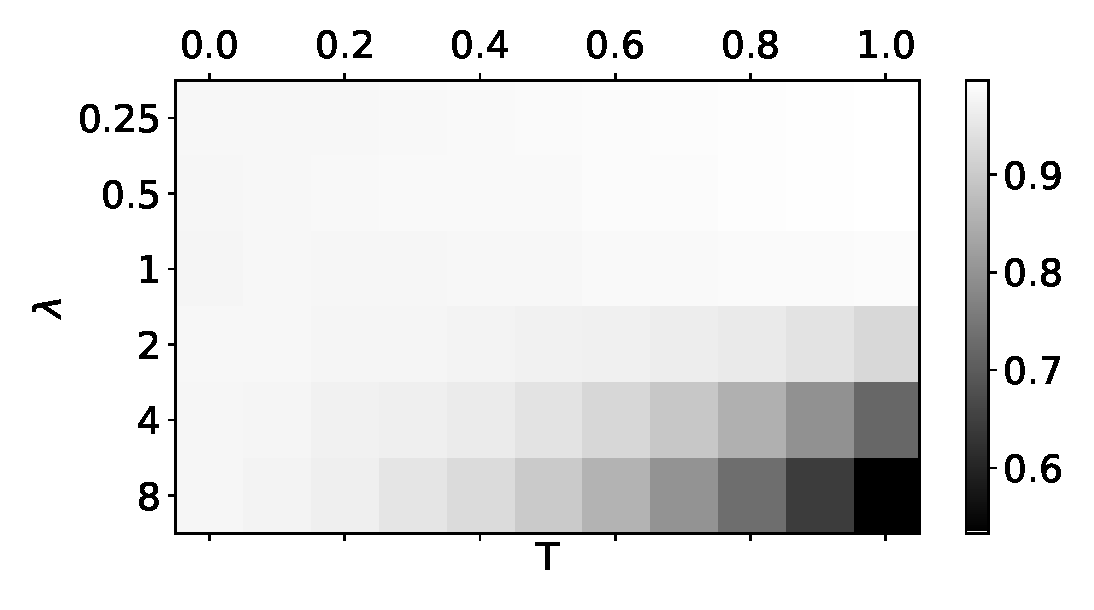
\includegraphics[width=1\textwidth]{figures/syn_T_lambda}
\caption{Вероятности классов для разных объектов.}
\label{fg:ex:synt:distr:lambda_T}
\end{figure}

Рассмотрим модель, которая учитывает информацию о истинных распределениях на классах для каждого объекта. Для этого будем минимизировать первые три слагаемых в формуле~\eqref{eq:st:class:1}, при~$T_0=1$ и~$\lambda=0{,}75$. В качестве меток учителя~$s_{i,k}$ использовались истинные вероятности для каждого класса для данного объекта. На рис~\ref{fg:ex:synt:distr:with} показано распределение, которое дала модель в данном случае, видно, что распределения являются сглаженными и концентрации всей вероятности в одном классе не наблюдается.

Заметим, что в данном примере предполагается, что модель учителя учитывает не только метки классов, а и распределение на метках классов, в то время как в выборке~$\mathcal{D} = \{\mathbf{X}, \mathbf{y}\},$ имеются только точечные оценки в виде меткок. 

В данном примере используются истинные распределения в качестве предсказаний учителя, но их можно заменить предсказаниями модели учителя, которая предсказывает не только сами меток, а и их распределение для каждого объекта.

На рис.~\ref{fg:ex:synt:distr:lambda_T} показана зависимость вероятности верного класса от температуры~$T$ и параметра доверия~$\lambda$ для одного из объекта из тестовой выборке. Видно, что при увеличении темпертуры распределение на классас становится более равномерным.

\subsection{Выборка Twitter Sentiment Analysis}
В данной части проводится эксперимент на выборке Twitter Sentiment Analysis. Данная выборка содержит короткие сообщения, для которых нужно предсказать эмоциональный окрас: содержит твит позитивный окрас или негативный. Выборка разделена на~$1{,}18$ миллиона твитов для обучения и~$0{,}35$ миллиона твитов для тестирования. В твитах была выполнена следующая предобработка:
\begin{itemize}
	\item все твиты были переведены в нижний регистр;
	\item все никнеймы вида~``@andrey'' были заменены на токен ``name'';
	\item все цифры были заменены на токен ``number''.
\end{itemize}
В качестве модели учителя использовалась модель Bi-LSTM с~$170$ тысячами параметров для обучения. В качестве эмбедингов обучалась матрица из~$30$ миллионов параметров в единой процедуре с моделью BI-LSTM. Обученная модель предсказывает с точностью~$0{,}835$. В качестве модели ученика рассматривается модель с $1538$ параметрами, но в качестве эмбедингов рассматривается переобученная модель BERT. Результаты данной части эксперимента показаны в табл.~\ref{tb:ce:1}.


\section{Выводы}
\begin{table}[]
\begin{center}
\begin{tabular}{|l|l|c|c|c|}
\hline
\multicolumn{1}{|c|}{Dataset} & \multicolumn{1}{c|}{Model} & CrossEntropyLoss      & Accuracy    &   StudentSize   \\ \hline
\multirow{2}{*}{FashionMnist} & without teacher    &  $0{,}461 \pm 0{,}005$ & $0{,}841\pm 0{,}002$ & 7850 \\ \cline{2-5} 
                              & with teacher       & $0{,}453 \pm 0{,}003$ & $0{,}842 \pm 0{,}002$ & 7850\\ \hline
\multirow{2}{*}{Synthetic}    & without teacher    & $0{,}225 \pm 0{,}002$ & $0{,}831\pm 0{,}002$ & 33 \\ \cline{2-5} 
                              &  with teacher       & $0{,}452 \pm 0{,}001$   & $0{,}828\pm 0{,}001$ & 33 \\ \hline
\multirow{2}{*}{Twitter }    & without teacher    & $0{,}501 \pm 0{,}006$ & $0{,}747\pm 0{,}005$ & $1538$  \\ \cline{2-5} 
                              &with teacher       & $0{,}489 \pm 0{,}003$   & $0{,}764\pm 0{,}004$ & $1538$ \\ \hline
\end{tabular}
\caption{Сводная таблица результатов вычислительного эксперимента.}
\label{tb:ce:1}
\end{center}
\end{table}

В данной работе проанализирована задача обучения модели ученика используя модель учителя.
Исследован метод дистилляции модели учителя в модель ученика.
В работе предложено вероятностное обоснования дистилляции, которое было предложено в работах~\cite{Hinton2015, Lopez2016}.
Введены вероятностные предположения, которые описывают дистилляцию моделей.
В рамках данных вероятностных предположений получен анализ некоторых моделей. Результат анализа сформулирован в виде теоремы~\ref{theorem:st:dist} и теоремы~\ref{theorem:st:reg}.

В рамках теоремы~\ref{theorem:st:reg} показано, что обучения линейной регрессии с учителем эквивалентно замене обучающей выборке и вероятностных предположений о распределении истинных ответов. Для задачи классификации ответы учителя дают дополнительную информацию в виде распределения классов для каждого объекта из обучающей выборки. Данная информация не может быть переписана в виде классической задачи классификации. Для использования данной информации требуется использовать распределение, которое представлено в теореме~\ref{theorem:st:dist}.

Анализ задачи регрессии в вычислительном эксперименте не проводится, так как в теореме~\ref{theorem:st:reg} была показана эквивалентность классическому решению задачи линейной регрессии. Для задачи классификации проведен вычислительный эксперимент. В вычислительном эксперименте сравнивается модель ученика, которая обучена без использования учителя и с использованием модели учителя. В таблице~\ref{tb:ce:1} показаны результаты вычислительного эксперимента для разных выборок. Из таблицы видно, что точность аппроксимации выборки учеником улучшается при использовании модели учителя.

В дальнейшем предполагается обобщить метод описаный в пункте~$4$ используя Байесовский подход выбора моделей машинного обучения. Также в рамках байесовсокго подхода планируется улучшить методы для получения улучшения качества не только для задачи классификации, а и для задачи регрессии.

\begin{thebibliography}{99}
\bibitem{LeCun1989}
	\textit{Y. LeCun, B. Boser, J. S. Denker, D. Henderson, R. E. Howard, W. Hubbard and L. D. Jackel} Backpropagation Applied to Handwritten Zip Code Recognition // Neural Computation. 1989. Vol.1 No 4. pp. 541--551.
\bibitem{Schmidhuber1997}
	\textit{Sepp Hochreiter; Jürgen Schmidhuber} Long short-term memory // Neural Computation. 1997. Vol. 9, No 8.  pp. 1735--1780.
\bibitem{Kaiming2015}
	\textit{Kaiming He, Xiangyu Zhang, Shaoqing Ren, Jian Sun} Deep Residual Learning for Image Recognition // CoRR. 2015
\bibitem{Vaswani2017}
	\textit{Ashish Vaswani, Noam Shazeer, Niki Parmar, Jakob Uszkoreit, Llion Jones, Aidan N. Gomez, Lukasz Kaiser, Illia Polosukhin} Attention Is All You Need // CoRR. 2017
\bibitem{Devlin2018}
	\textit{Jacob Devlin, Ming-Wei Chang, Kenton Lee, Kristina Toutanova} BERT: Pre-training of Deep Bidirectional Transformers for Language Understanding // arXiv preprint arXiv:1810.04805. 2018
\bibitem{Vapnik2015}
	\textit{Vladimir Vapnik, Rauf Izmailov} Learning Using Privileged Information: Similarity Control and Knowledge Transfer // Journal of Machine Learning Research. 2015. No 16. pp. 2023--2049.
\bibitem{Lopez2016}
	\textit{David Lopez-Paz, Leon Bottou, Bernhard Scholkopf, Vladimir Vapnik} UNIFYING DISTILLATION
AND PRIVILEGED INFORMATION // Published as a conference paper at ICLR. 2016.
\bibitem{Hinton2015}
        \textit{Geoffrey Hinton, Oriol Vinyals, jeff Dean} Distilling the Knowledge in a Neural Network // NIPS Deep Learning and Representation Learning Workshop. 2015.
\bibitem{mnist}
	\textit{LeCun Y.,  Cortes C., Burges C.} The MNIST dataset of handwritten digits, 1998. \url{http://yann.lecun.com/exdb/mnist/index.html}
\bibitem{fashionmnist}
	\textit{Han Xiao and Kashif Rasul and Roland Vollgraf} Fashion-MNIST: a Novel Image Dataset for Benchmarking Machine Learning Algorithms // arXiv, 2017.
\bibitem{kingma2014}
	\textit{Diederik P. Kingma and Jimmy Ba} Adam: A Method for Stochastic Optimization // arXiv, 2014.
\bibitem{bachteev2018}
	\textit{О.\,Ю. Бахтеев, В.\,В. Стрижов} Выбор моделей глубокого обучения субоптимальной сложности // Автоматика и телемеханика, 2018.
\bibitem{twiter2013}
	\textit{Theresa Wilson, Zornitsa Kozareva, Preslav Nakov, Sara Rosenthal, Veselin Stoyanov, and Alan Ritter} SemEval-2013 task 2: Sentiment analysis in twitter // In Proceedings of the International Workshop on Semantic Evaluation, SemEval ’13. 2013.
 \end{thebibliography}


\end{document}

